\documentclass[a4paper,12pt]{article}
\usepackage[left = 1.5cm, top = 2cm, right = 1.5cm, bottom = 2cm]{geometry}

\usepackage{graphicx}
\usepackage{booktabs}
\usepackage{caption}
\usepackage{amsmath}
\usepackage{amsfonts}
\usepackage{amsthm}
\usepackage{changepage}
\usepackage{amssymb}
\usepackage{subcaption}
\usepackage{float}
\usepackage[dvipsnames]{xcolor}
\usepackage[most]{tcolorbox}
\usepackage[shortlabels]{enumitem}
\usepackage{pdfpages}
\usepackage{braket}
\usepackage{tikz}

\usepackage{verbatim}
\usepackage[noend,ruled,linesnumbered]{algorithm2e}
\DontPrintSemicolon
\SetKwInOut{Input}{Input}
\SetKwInOut{Output}{Output}

% Custom commands
\newcommand{\algo}[1]{\emph{\textcolor{blue}{#1}}}
\newcommand{\xor}{\oplus}
\newcommand{\ord}{\text{ord}}
\newcommand{\horiline}{
\noindent\makebox[\linewidth]{
    \rule{\paperwidth}{0.4pt}}
}
\newcommand{\bfhoriline}{
\noindent\makebox[\linewidth]{
    \rule{\paperwidth}{2pt}}
}
\newcommand{\ay}{\mathcal{A}}
\newcommand{\bee}{\mathcal{B}}
\newcommand{\Z}{\mathbb{Z}}
\newcommand{\R}{\mathbb{R}}
\newcommand{\E}[1]{\mathbb{E}\left[ #1 \right]}
\newcommand{\keygen}{\operatorname{KeyGen}}
\newcommand{\enc}{\operatorname{Enc}}
\newcommand{\dec}{\operatorname{Dec}}
\newcommand{\pk}{\operatorname{PK}}
\newcommand{\sk}{\operatorname{SK}}
\newcommand{\green}[1]{\mathcolor{PineGreen}{#1}}
\newcommand{\red}[1]{\mathcolor{red}{#1}}
\newcommand{\blue}[1]{\mathcolor{blue}{#1}}
\newcommand{\mat}[1]{\begin{bmatrix} #1 \end{bmatrix}}
\newcommand{\pmat}[1]{\begin{pmatrix} #1 \end{pmatrix}}
\newcommand{\abs}[1]{\left| #1 \right|}
\newcommand{\norm}[1]{\left\Vert #1 \right\Vert}
\newcommand{\Zmod}[1]{\mathbb{Z}/ #1 \mathbb{Z}}
\newcommand{\Zmodstar}[1]{(\Zmod{ #1 })^*}
\newcommand{\rank}{\operatorname{rank}}
\newcommand{\spank}{\operatorname{span}}
\newcommand{\pderiv}[2]{\frac{\partial #1}{\partial #2}}
\newcommand{\lcm}{\operatorname{lcm}}
\newcommand{\tr}{\operatorname{tr}}

% Custom spacings
\setlength\parindent{0pt}
\setlength{\parskip}{0.75em}

% Custom environemnts
% \begin{lemma} or \begin{lemma}[Case 1: ...] for an underlined heading
\newenvironment{lemma}[1][]
    {\ifstrempty{#1}{}{\underline{#1}\par\nobreak\vspace{0.25em}}%
     \begin{adjustwidth}{1cm}{0cm}}
    {\end{adjustwidth}}



% Beamer-style titled blocks
\definecolor{blocktitle}{RGB}{34,45,120}
\definecolor{blockbody}{RGB}{230,231,243}
\tcbset{blockstyle/.style={
    enhanced, breakable,
    colback=blockbody, colbacktitle=blocktitle, coltitle=white,
    colframe=blocktitle, boxrule=0pt, arc=2pt,
    left=6pt, right=6pt, top=4pt, bottom=4pt,
    fonttitle=\bfseries,
    after skip=1.5em,
    before upper={\setlength{\parskip}{0.6em}}, % restore inter-paragraph gap
}}

% \niceblock[<extra tcolorbox options>]{<title>}{<body>}
%   \niceblock{Theorem 1 (Fermat)}{...}
%   \niceblock[colbacktitle=PineGreen, colframe=PineGreen]{Exercise 2}{...}
\newtcolorbox{niceblockenv}[1][]{blockstyle, #1}
\newcommand{\niceblock}[3][]{%
    \begin{niceblockenv}[title={#2}, #1]%
    #3%
    \end{niceblockenv}%
}

% Same block without a title bar, and for bodies that \niceblock cannot take as
% an argument (verbatim, \begin{comment}, ...):
%   \begin{niceblockenv}[title={Theorem 1}] ... \end{niceblockenv}

% Numbered, cross-referenceable blocks. All kinds share one counter, so numbers
% are unique: Definition 1.1, Theorem 1.2, Exercise 1.3, ... (reset each section).
\newcounter{niceblockcounter}

% \newniceblock{<cmd>}{<Heading>}{<extra tcolorbox options>}
%   defines \<cmd>[<options>]{<name>}{<body>} and the environment <cmd>env
\newcommand{\newniceblock}[3]{%
    \newtcolorbox[use counter=niceblockcounter, number within=section]{#1env}[2][]{%
        blockstyle,
        title={#2~\thetcbcounter\ifstrempty{##2}{}{: ##2}},
        #3, ##1%
    }%
    \expandafter\newcommand\csname #1\endcsname[3][]{%
        \begin{#1env}[##1]{##2}##3\end{#1env}%
    }%
}

% Usage: \definition[label=def:shannon]{Shannon Entropy}{...} -> "Definition 1.1: Shannon Entropy"
%        \theorem{}{...}                                      -> "Theorem 1.2" (no name)
% then refer to it anywhere with \ref{def:shannon}.
% NOTE: \newniceblock{lemma}{Lemma} would clash with the lemma environment above.
\newniceblock{definition}{Definition}{}
\newniceblock{theorem}{Theorem}{}
\newniceblock{exercise}{Exercise}{colbacktitle=PineGreen, colframe=PineGreen,
    segmentation style={solid, PineGreen, line width=0.6pt}}

% Message arrows for two-party game diagrams (challenger / adversary).
% The \makebox sets a minimum arrow length so short labels still look right.
\newcommand{\msgto}[1]{\xrightarrow{\makebox[2.2cm]{$\scriptstyle #1$}}}
\newcommand{\msgfrom}[1]{\xleftarrow{\makebox[2.2cm]{$\scriptstyle #1$}}}

% Styles for the Alice--Bob--Eve channel diagrams. Parties reuse the block
% colours; anything belonging to the adversary is red.
\usetikzlibrary{arrows.meta, positioning, calc, fit, backgrounds}
\tikzset{
    party/.style={draw=blocktitle, fill=blockbody, rounded corners=2pt,
        line width=0.8pt, inner sep=6pt, font=\bfseries, minimum width=1.5cm},
    adversary/.style={party, draw=red!65!black, fill=red!8},
    blackbox/.style={draw=red!65!black, fill=red!8, rounded corners=2pt,
        line width=0.8pt, inner sep=6pt, minimum width=1.5cm},
    wire/.style={-{Stealth[length=2.2mm]}, line width=0.8pt},
    leak/.style={wire, densely dashed, red!65!black},
    wirelab/.style={font=\small, inner sep=2pt},
    note/.style={font=\scriptsize\itshape, inner sep=2pt},
    region/.style={draw=red!65!black, densely dotted, rounded corners=4pt,
        inner sep=10pt, line width=0.7pt},
}

%============================================%
%============= Useful Structures ============%
%============================================%

%====== Table %======%

% \begin{table}[H]
%     \centering
%     \caption{--}
%     \label{tab:my_table}
%     \begin{tabular}{@{} l c c @{}}
%         \toprule
%         \textbf{--} & \textbf{--} & \textbf{--} \\
%         \midrule
%         -- & -- & -- \\
%         -- & -- & -- \\
%         -- & -- & -- \\
%         \bottomrule
%     \end{tabular}
% \end{table}

%====== Figure %======%

% \begin{figure}[H]
%     \centering
%     \includegraphics[width=0.6\linewidth]{figure.png}
%     \caption{--}
%     \label{fig:my_figure}
% \end{figure}

%====== a,b,c enumerate %======%

% \begin{enumerate}[a)]
%     \item First part
%     \item Second part
% \end{enumerate}


\usepackage{hyperref} % hyperref package (should be loaded last)

\hypersetup{breaklinks=true,colorlinks,linkcolor=blue,urlcolor=blue,pdfpagemode=UseNone}

\begin{document}

\subsection{Distinguishability}

In this section we concern ourselves with \emph{distinguishing} problems.
That is, if we have two quantum states $\rho$ and $\sigma$, when and how can we tell them apart?

First, lets consider what it means for two states to be \emph{indistinguishable}.
Formally, we write:
\definition{Indistinguishability}{
    Two quantum states are said to be \emph{indistinguishable} if, for any measurement procedure, the probability distribution of outcomes is identical between the two states.
}

This should make intuitive sense; if we can't construct \emph{any} procedure to tell these states apart, how could we possibly distinguish them?
We don't even consider such states to different states.

As cryptographers, this definition should feel very familiar.
We can view the indistinguishability of quantum states as a game, similar to your IND-{*} security definitions:

\begin{figure}[H]
    \centering
    \begin{tabular}{@{} l c l @{}}
        \multicolumn{1}{@{}c}{\textbf{Challenger}} & &
        \multicolumn{1}{c@{}}{\textbf{Adversary}} \\[0.8em]

        & $\msgto{\rho_0,\ \rho_1}$ & [knows both descriptions] \\[0.8em]

        $b \overset{\$}{\leftarrow} \{0,1\}$ & & \\[0.4em]
        $\tau \leftarrow \rho_b$
        & $\msgto{\tau}$ & [any measurement $\mathcal{M}$] \\[0.8em]

        & $\msgfrom{b'}$ & outputs $b' \leftarrow \mathcal{M}(\tau)$ \\
    \end{tabular}
    \caption{The indistinguishability game. The adversary wins if $b' = b$.}
    \label{fig:indgame}
\end{figure}

The quantum states $\rho_0$ and $\rho_1$ in Figure~\ref{fig:indgame} are indistinguishable if and only if the best adversary can only win with probability $1/2$.

We can consider 2 more categories: \emph{distinguishable} states are pairs of states that are not indistinguishable, and \emph{perfectly distinguishable} states are pairs of states where there is a measurement procedure that is guaranteed to succeed.
You can think of \emph{perfectly distinguishable} as states where there exists an adversary which always wins.

Let's try to classify some pairs of states we've seen before:
\exercise{Distinguishing states}{
    \begin{enumerate}
        \item Are the $\ket{0}$ and $\ket{1}$ states distinguishable?
        \item What about the states $\ket{+}$ and $\begin{cases}\ket{0} & \text{with prob. }1/2 \\ \ket{1} & \text{with prob. }1/2\end{cases}$ \quad ?
        \item What about the states $\begin{cases}\ket{0} & \text{with prob. }1/2 \\ \ket{1} & \text{with prob. }1/2\end{cases}$ and $\begin{cases}\ket{+} & \text{with prob. }1/2 \\ \ket{-} & \text{with prob. }1/2\end{cases}$\quad?
    \end{enumerate}
    \tcblower
    \textit{Answers}
    \begin{enumerate}
        \item Yes. To do this, we measure our unknown state in the computational basis. If it is $\ket{0}$, we will measure $0$ with unit probability, and vice versa. So we can \emph{always} succeed, and these states are perfectly distinguishable.
        \item Yes. Repeating the above won't work (why?), but we can use the $\{\ket{+},\ket{-}\}$ basis and guess $\ket{+}$ if and only if we measure the state to be $\ket{+}$. If $\ket{+}$ is sent, our measurement is perfect and we will guess correct. If the other state is sent, we measure $\ket{+}$ and $\ket{-}$ with equal probability, and will be wrong if we guess. 
        So the success probability of our strategy is $1/2 + 1/4=3/4$ which is greater than $1/2$.
        Can you come up with a \emph{better} strategy? Does a \emph{perfect} strategy exist?
        \item No. Expanding our density matrices yields the same for both:
        \begin{flalign*}
            \frac{1}{2}\mat{1 \\ 0}\mat{1 & 0} + \frac{1}{2}\mat{0 \\ 1}\mat{0 & 1}
            = \frac{1}{2}\mat{1 & 0 \\ 0 & 0} + \frac{1}{2}\mat{0 & 0 \\ 0 & 1}
            &= \frac{1}{2}\mat{1 & 0 \\ 0 & 1} \\
            \frac{1}{4}\mat{1 \\ 1}\mat{1 & 1} + \frac{1}{4}\mat{1 \\ -1}\mat{1 & -1}
            = \frac{1}{4}\mat{1 & 1 \\ 1 & 1} + \frac{1}{4}\mat{1 & -1 \\ -1 & 1}
            &= \frac{1}{2}\mat{1 & 0 \\ 0 & 1} \\
        \end{flalign*}
        We can then model any transformations and measurements purely on our unknown state as a function of its density matrix.
        It must therefore be impossible to construct a procedure that distinguishes these!
    \end{enumerate}
}

To characterize these categories, we can use the notion of \emph{trace distance}.

\subsubsection{Trace distance}
Start with a definition of the trace-norm:
\definition{Trace norm}{
    For a normal matrix $M$, the trace norm of M is defined as
    $$\norm{M}_1 = \tr\left(\abs{M}\right) = \tr\left(\sqrt{M^*M}\right)$$ 
}
In this notation, the $\abs{\cdot}$ and $\sqrt{\cdot}$ functions are being applied to the eigenvalues of the spectral decomposition of $M$. In other words, to apply such a function $f: \mathbb{C} \to \mathbb{C}$ to $M$ involves
$$
f(M)=U\mat{
    f(\lambda_1) & 0 & \cdots &  0 \\
    0 & f(\lambda_2) & \cdots & 0 \\
    0 & \vdots & \ddots & \vdots \\
    0 & 0 & \cdots & f(\lambda_d)
}U^*
$$
using $M$'s spectral decomposition.

Using this notion, define the trace distance as follows:
\definition{Trace Distance}{
    Let $\rho,\sigma$ be the density operators for two quantum states. The trace distance between these states is defined as:
    $$\norm{\rho-\sigma}_1$$
}
Note that some sources like the Nielsen and Chuang textbook add a factor of $1/2$ for the trace distance. Instead, we follow the QIC 710 course notes, which omit this.

This is an example of a \emph{distance metric}, because it seeks to answer the question ``how \emph{close} are two quantum states''?
The natural question you'd have about this is what we mean by \emph{``close''} here.
In fact, this notion of distance is directly related to our adversary's advantage in the indistinguishability game!
This is proved by The Holevo-Helstrom Theorem.

\subsubsection{The Holevo-Helstrom Theorem}

\theorem{Holevo-Helstrom Theorem}{
    Let $\rho_0$ and $\rho_1$ be the density matrices of two $d$-dimensional quantum states. If one of these two states is prepared by the flip of a fair coin then the best distinguishing procedure succeeds with probability
    $$\frac{1}{2} + \frac{1}{4}\norm{\rho_0 - \rho_1}_1$$
}

Let's use this on our previous examples:
\exercise{Trace distance and distinguishability}{
    Find the trace distance between:
    \begin{enumerate}
        \item The states $\ket{0}$ and $\ket{1}$
        \item The states $\ket{+}$ and $\begin{cases}\ket{0} & \text{with prob. }1/2 \\ \ket{1} & \text{with prob. }1/2\end{cases}$
        \item The states $\begin{cases}\ket{0} & \text{with prob. }1/2 \\ \ket{1} & \text{with prob. }1/2\end{cases}$ and $\begin{cases}\ket{+} & \text{with prob. }1/2 \\ \ket{-} & \text{with prob. }1/2\end{cases}$
    \end{enumerate}
    \tcblower
    \textit{Answers}
    \begin{enumerate}
        \item We have density matrices of $\mat{1 & 0 \\ 0 & 0}$ and $\mat{0 & 0 \\ 0 & 1}$, which gives a trace distance:
        $$\norm{\mat{1 & 0 \\ 0 & 0} - \mat{0 & 0 \\ 0 & 1}}_1 = \norm{\mat{1 & 0 \\ 0 & -1}}_1 = \abs{1} + \abs{-1} = 2$$
        which confirms the fact these states are perfectly distinguishable!
        \item Now, we have density matrices $\ket{+}\bra{+} = \frac{1}{2}\mat{1 & 1 \\ 1 & 1}$ and $\frac{1}{2}\mat{1 & 0 \\ 0 & 1}$, whose difference is
        $$\frac{1}{2}\mat{1 & 1 \\ 1 & 1} - \frac{1}{2}\mat{1 & 0 \\ 0 & 1} = \frac{1}{2}\mat{0 & 1 \\ 1 & 0}$$
        Unlike the previous part, this difference is \emph{not} diagonal, so we cannot simply add up the absolute values of the entries along its diagonal. The trace norm is the sum of the absolute values of the \emph{eigenvalues}, which here are $\pm\frac{1}{2}$:
        $$\norm{\frac{1}{2}\mat{0 & 1 \\ 1 & 0}}_1 = \abs{\frac{1}{2}} + \abs{-\frac{1}{2}} = 1$$
        By the Holevo-Helstrom theorem, the best distinguishing procedure succeeds with probability $\frac{1}{2} + \frac{1}{4}(1) = \frac{3}{4}$. This is exactly the success probability of the strategy we found by hand earlier! So that strategy was already optimal and no perfect strategy exists.
        These states are therefore distinguishable but not \emph{perfectly} distinguishable.
        \item This one is easy. Since our density matrices are the same, we have that the trace distrance is $\norm{\rho-\rho}_1=\norm{\mathcal{O}}_1=0$.
        This confirms the last conclusion that these states are indistinguishable!
    \end{enumerate}
}


\section{Entropy, information, and basic security intuition}

\subsection{A Motivating Example}

To motivate our discussion of quantum information theory, we can ``dream'' a bit about what might be possible in sharing quantum information.
Let's start with a real setting: Alice wants to send Bob a secret over some channel.
The goal is to prevent as much of the message being leaked as possible.

\begin{figure}[H]
    \centering
    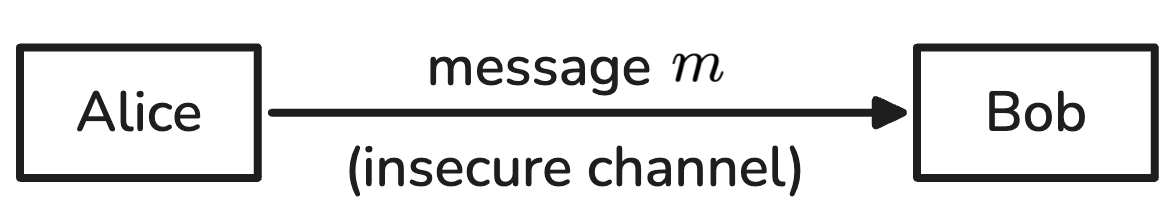
\includegraphics[width=0.55\linewidth]{diagrams/1.png}
\end{figure}

Now imagine that a third party, Eve, is listening in.

\begin{figure}[H]
    \centering
    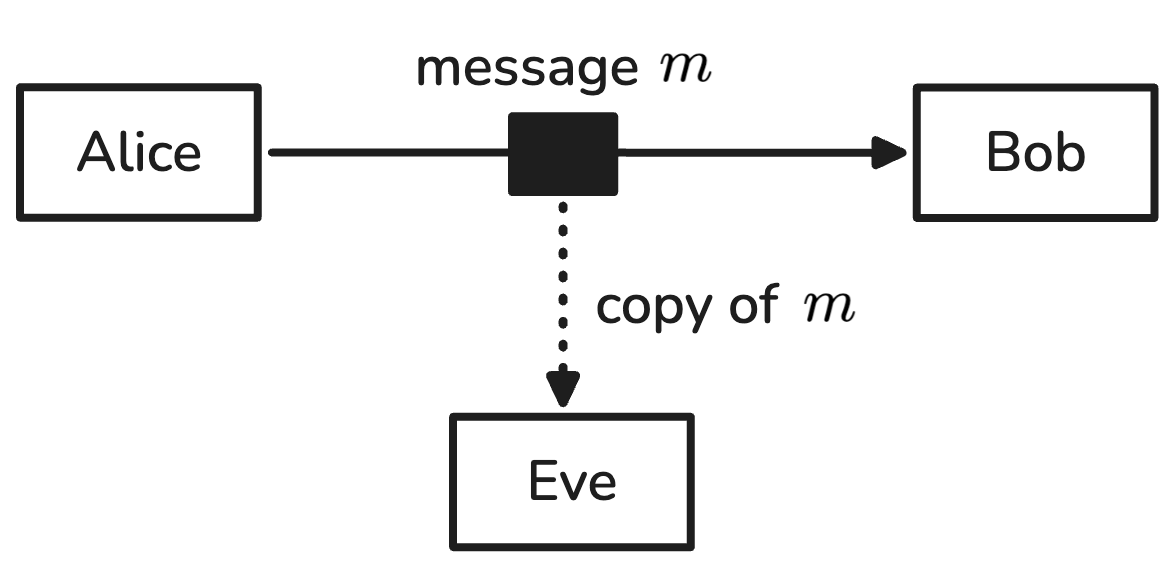
\includegraphics[width=0.55\linewidth]{diagrams/2.png}
\end{figure}

In a classic setting, there isn't anything we can do to stop Eve from listening to the communications between Alice and Bob.
It's next to impossible to even tell if someone is listening at all.
Our only hope is to rely on public-key encryption to render the message indecipherable, \emph{contingent on some hardness assumption}.

Now, lets start dreaming about what this same interaction might look like in a quantum setting.
Suppose that Alice finds a way to encode this secret into a quantum state, say $\ket{\psi}$. 

\begin{figure}[H]
    \centering
    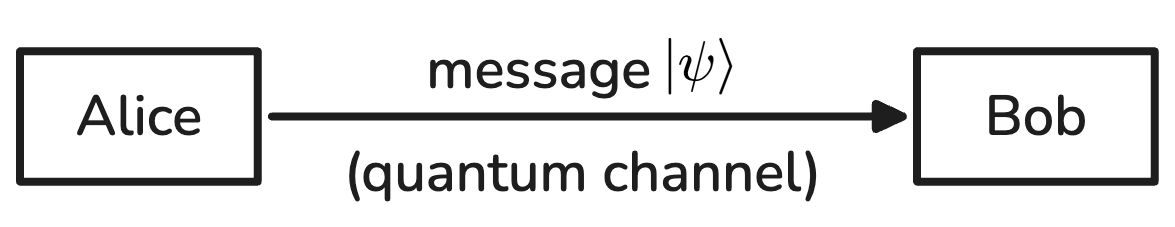
\includegraphics[width=0.55\linewidth]{diagrams/3.png}
\end{figure}

Let's take Eve's perspective.
In order to secretly extract information, we can suppose that Eve hopes to perform some kind of interaction with Alice's secret state $\ket{\psi}$ with some buffer state $\ket{u}$, which will modify only $\ket{u}$ and leave $\ket{\psi}$ unchanged.

\begin{figure}[H]
    \centering
    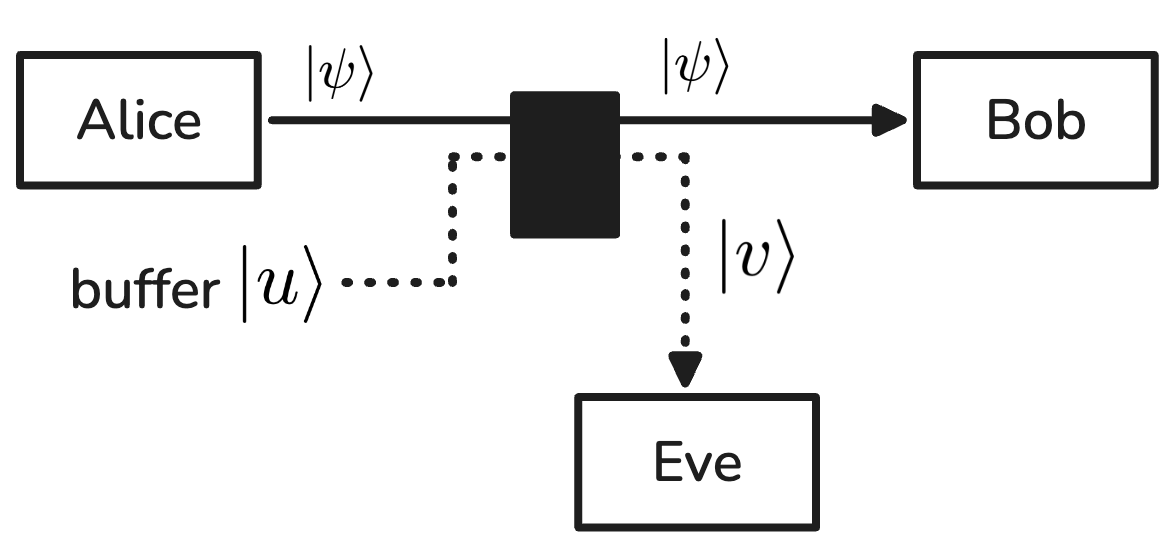
\includegraphics[width=0.55\linewidth]{diagrams/4.png}
\end{figure}

The idea here is that the output $\ket{v}$ will contain information about the state $\ket{\psi}$, which can be then measured without affecting $\ket{\psi}$ itself.
If this output $\ket{v}$ depends on $\ket{\psi}$, it should change if $\ket{\psi}$ was substituted with some other non-orthogonal state $\ket{\varphi}$. So assume $\ket{v}\ne\ket{v'}$.

In summary, we have:
\begin{align*}
    \ket{\psi}\ket{u} &\to \ket{\psi}\ket{v} \\
    \ket{\varphi}\ket{u} &\to \ket{\varphi}\ket{v'} \\
    \intertext{we can model this pure-state transformation using a unitary transformation $U$:}
    U\ket{\psi}\ket{u} &= \ket{\psi}\ket{v} \\
    U\ket{\varphi}\ket{u} &= \ket{\varphi}\ket{v'} \\
    \intertext{taking the inner product of these two equations yields}
    \bigl(\bra{\varphi}\otimes\bra{u}\bigr) U^\dagger U \bigl(\ket{\psi}\otimes\ket{u}\bigr)
        &= \bigl(\bra{\varphi}\otimes\bra{v'}\bigr)\bigl(\ket{\psi}\otimes\ket{v}\bigr) \\
    \implies \braket{\varphi|\psi}\braket{u|u} &= \braket{\varphi|\psi}\braket{v'|v} \\
    \implies \braket{v'|v} &= 1
\end{align*}
which means $\ket{v'}$ and $\ket{v}$ must be identical, reaching contradiction!
So it seems that Eve's job is made impossible; they cannot eavesdrop while preserving the message $\ket{\psi}$!
This example illustrates the principle that \emph{information gain implies disturbance}:
\theorem{Information gain implies disturbance}{
    In any attempt to distinguish between two non-orthogonal quantum states, information gain is only possible at the expense of introducing disturbance to the signal.
}

Still, this result is all or nothing.
If Eve is allowed to disturb the signal just a \emph{little}, does that necessarily imply that they can only gain a \emph{little} information?
In order to answer questions like these, we need a way to quantify information and uncertainty, which leads us to information theory.

\subsection{Introduction to Entropy}

``Entropy'' is a very overloaded term with a range of different meanings across and within different domains of math and science.
% owaldron TODO include some examples
Even in our discussions, different kinds of entropy are used to perform different measures.
The goal for today is to understand some basic entropies to get an idea of how it can be used to ``quantify and amound of information''.

\subsubsection{Shannon entropy}

A particularly useful (and famous) entropy is the Shannon entropy:
\definition[label=def:shannon]{Shannon entropy}{
    For a discrete, random variable $X=1,...,n$ with probability distribution $p_1,...,p_n$, the Shannon entropy is defined as:
    $$H(X) \equiv H(p_1, ..., p_n)\equiv-\sum_x p_x \log p_x$$
}
The one caveat is that if $p_x=0$, then we neglect the term by agreeing $0\log 0 \equiv 0$. Intuitively, if $p_x=0$, then $X$ can never take the value of $x$, so why should this case affect the entropy!

Something else to notice is that the entropy $H(X)$ does not depend on the labels of what $X$ can take, and is only a function of its distribution.

Let's play with this a little bit:
\exercise{Playing with Shannon entropy}{
    \begin{enumerate}
        \item What is the entropy associated with the toss a fair coin?
        \item What is the entropy associated with the roll of a fair die?
        \item What is the entropy associated with the roll of a \emph{Mario die} (with sides 1,3,3,3,5,6)? What about a \emph{Peach die} (0,2,4,4,4,6)?
        \item How do the above compare to a fair 4-sided die?
    \end{enumerate}
}

So we understand how to calculate Shannon entropy, but what is the intuition behind it representing a quantity of information?
One answer is that it captures \emph{the physical resources needed to communicate information}.

Suppose we have an information source, which is constantly producing i.i.d. discrete random variables $X_1,X_2,...$.
What is the expected amount of minimal physical ressources we need to send, on average, so that this string of random variables can be perfectly reconstructed by the receiver?
The answer, amazingly, is $H(X)=H(X_1)=H(X_2)...$ bits!

\subsubsection{Conditional entropy \& mutual information}

Now, consider if we have a pair of random variables $X,Y$ that may or may not be related in some way.
Let's see how we can quantify the relationship between the information content of $X$ and the information content of $Y$.

For starters, we know that we can consider the \emph{joint distribution} by treating the pair $(X,Y)$ as a single random variable with a single (joint) distribution.
The respective \emph{joint entropy} of this distribution is naturally:
$$H(X,Y) \equiv  -\sum_{x,y}p(x,y)\log p(x,y)$$
Now, consider the case where we already know the value of $Y$.
This means we've acquired $H(Y)$ bits of information about the pair $(X,Y)$.
Any information remaining about $(X,Y)$ is due to our uncertainty regarding $X$.
So, we define the \emph{entropy of $X$ conditional on knowing $Y$} is intuitively:
$$H(X|Y) \equiv H(X,Y) - H(Y)$$
Now, consider the sum $H(X)+H(Y)$.
This encompasses the unique information provided by $X$ and $Y$, as well as \emph{two times} the common information between $X$ and $Y$.
If we subtract off the total information from $X$ and $Y$, $H(X,Y)$, what remains will be the information common to $X$ and $Y$.
We call this quantity the \emph{mutual information content} of $X$ and $Y$, written
$$H(X:Y)=H(X) + H(Y) - H(X,Y)$$ 

In summary:
\definition{Conditional entropy and mutual information}{
    Let $X,Y$ be two random variables. The join entropy of $X$ and $Y$ is:
    $$H(X,Y) \equiv  -\sum_{x,y}p(x,y)\log p(x,y)$$
    the entropy of $X$ conditional on knowing $Y$ is
    $$H(X|Y)\equiv H(X,Y) - H(Y)$$
    and the mutual information of $X$ and $Y$ is
    $$H(X:Y)\equiv H(X) + H(Y) - H(X,Y)$$
}

Let's do a quick worked example.
Suppose we have two \emph{distinctly} unfair coins: a heads-heavy coin that lands heads with probability $0.9$, and a tails-heavy coin that lands heads with probability $0.1$.
We draw one of the two at random (fairly!), flip it once, and record what came up.
Let $X$ be which coin we drew, and let $Y$ be the outcome of the flip.
The joint distribution is then:
\begin{center}
    \begin{tabular}{@{} l c c @{}}
        \toprule
        $p(x,y)$ & $Y=\text{heads}$ & $Y=\text{tails}$ \\
        \midrule
        $X=$ heads-heavy & $0.45$ & $0.05$ \\
        $X=$ tails-heavy & $0.05$ & $0.45$ \\
        \bottomrule
    \end{tabular}
\end{center}
Both marginals are uniform: we drew the coin with a fair flip, so $H(X)=1$, and the two biases are mirror images of each other, so heads and tails are equally likely overall and $H(Y)=1$ as well.
The joint entropy is
$$H(X,Y) = -2\left(0.45\log 0.45\right) - 2\left(0.05\log 0.05\right) \approx 1.469$$
from which everything else follows:
$$H(Y|X) = H(X,Y) - H(X) \approx 0.469 \qquad H(X|Y) = H(X,Y) - H(Y) \approx 0.469$$
$$H(X:Y) = H(X) + H(Y) - H(X,Y) \approx 0.531$$

Let's read these off one at a time.
$H(Y|X)\approx0.469$ says that even once we know \emph{which} coin we are holding, the flip still carries about $0.47$ bits of uncertainty --- this is just the entropy of a single $0.9$-biased coin, the irreducible randomness of the flip itself.
$H(X|Y)\approx0.469$ says the same in reverse: after seeing the flip, about $0.47$ bits of uncertainty remain about which coin we drew.
And $H(X:Y)\approx0.531$ says the flip told us just over half a bit about the identity of the coin.
Not a whole bit (a single flip can never fully determine which coin we hold) but certainly more than nothing.

The ``distinctly unfair'' part is doing all the work here. In general, if the two coins have biases $p$ and $1-p$, the same computation gives
$$H(X:Y) = 1 - H(p)$$
so if both coins were fair ($p=1/2$) then $Y$ would be independent of $X$ and the flip would tell us \emph{nothing}: $H(X:Y)=0$.
Push the bias the other way to $p=0.99$ and we get $H(X:Y)\approx0.919$, so the flip almost completely gives away which coin we drew.

\subsection{The quantum analogue: von Neumann entropy}

What if we viewed a quantum state as a random variable storing information;
could we consider the entropy \emph{associated with this state}?
The answer is yes!
We can use a translation (of sorts) of Shannon entropy to study this.
This was invented by von Neumann as follows:

\definition{Von Neumann entropy} {
    For a quantum state $\rho$, the von Neumann entropy is defined as
    $$S(\rho) \equiv -\operatorname{tr}(\rho\log\rho)$$
}
That is the negative \emph{trace} of the matrix $\rho\log\rho$. This inner term is the matrix product between the density operator and the \emph{matrix logarithm} (ie. the matrix that satisfies $2^{log(\rho)}=\rho$ under matrix exponentiation via power series).
Because of these matrix operations, this expression isn't very useful on its own.
However, if we write $\lambda_x$ to be the eigenvalues of $\rho$, we can re-express this as:
$$S(\rho)=-\sum_x \lambda_x\log\lambda_x$$
taking again the convention that $0\log0 \equiv 0$.

Now we can work with this; lets go right into computing some examples:
\exercise{Computing von Neumann entropy}{
    \begin{enumerate}
        \item What is the von Neumann entropy of \emph{any} pure state $\ket{\psi}$?
        \item What is the von Neumann entropy of the state $\begin{cases}\ket{0} & \text{with prob. }1/2 \\ \ket{1} & \text{with prob. }1/2\end{cases}$ \quad ?
        \item What is the von Neumann entropy of the state $\begin{cases}\ket{0} & \text{with prob. }1/2 \\ \ket{+} & \text{with prob. }1/2\end{cases}$ \quad ? How does it compare to the previous answer?
    \end{enumerate}
}

\end{document}



